\section{Time Transactions}
\label{section:time_transactions}

\begin{figure}[H]
\centering
\includegraphics[scale=0.60]{05_time_transactions/png/time_transaction}
\caption{Time Transactions}
\label{fig:time_transactions2}
\end{figure}

\subsection{Including Time Transactions in Our Model}

\begin{figure}[H]
\centering
\includegraphics[scale=0.60]{05_time_transactions/png/time_transaction_feedback_schema}
\caption{Exchange and Time Transaction Feedback Schema}
\label{fig:exchange_and_time_transaction_schema1}
\end{figure}

In Section \ref{section:exchange_transactions_and_errors} we showed that there is a bound on the set of
economic transactions that are possible, and that the error bound is determined by $H$ (which we can
consider as beyond out control), the inflation rate $I$ and the growth rate $G$. We can control the
inflation rate, but in general the growth rate is external to our control. We also showed that to
achieve the goals of our currency requires a positive inflation rate. The unit in which we write
prices is continuously changing. The unit used to denominate payments in contracts is generally this
price unit. We show that this method of choosing interest rates is undercontrollable as discussed in
Section \ref{section:system_specification} such that under conditions of a positive rate of change
in the inflation rate, i.e. when

\[
    \frac {\Delta I} I > 0
\]

then either the real costs of borrowing must increase or the output $Q$ must decrease. Based on   
Figure \ref{fig:ui_bound} this results in unemployment/inflation tracking that appears as indicated
in Figure \ref{fig:uncontrollability_problem}.

\begin{figure}[H]
\centering
\includegraphics[scale=0.48]{05_time_transactions/png/interest_inflation_coupling1}
\caption{Interest-Inflation Coupling}
\label{fig:interest_inflation_coupling}
\end{figure}

Control failure occurs until the rate of change in the inflation rate drops to zero or becomes
negative. The combination of the error bound and underspecification tracking leads to a fundamental
control problem. To set conditions where aggregate equilibrium is possible, the inflation rate must
be increased to region $D$ as shown in Figure \ref{fig:ui_bound}. As the inflation rate increases,
uncontrollability tracking reduces the growth rate, increases the unemployment rate. The solution to
this problem is to correct the units in which contracts are written. If a unit of account of
constant value is used, real interest rates can be trivially specified because the unit directly
measures real payments and so fully specifies our control problem. Given that a currency limits
transactions to exchange transactions and time transactions, and that a unit of account of constant
value is used, and given that there are no other unforseen destabilizing effects, the currency can
be controlled to maintain aggregate equilibrium. If a unit of account of constant value is not used,
it is not possible for a currency to maintain aggregate equilibrium.

\subsection{Interest Control Failure}

We showed in Section \ref{section:exchange_transactions_and_errors}. that the unit in which prices are
denominated must be continuously changing.

\begin{figure}[H]
\centering
\includegraphics[scale=0.48]{05_time_transactions/png/time_transaction}
\caption{Time Transactions}
\label{fig:time_transaction_contracts}
\end{figure}

This unit is used in time transactions to denominate the initial lending of currency, to denominate
the repayment, and it is also common practice to use it to specify the repayment in a contract.
Because this unit in continuously changing, the value written into contracts must be written in such
a way as to specify a real interest rate, i.e. an interest rate written in terms of purchasing
power. Fisher \cite{fisher1907} notes that in order to specify a real interest rate $r$ then the
value $i$ needs to be written into contracts, where

\[
    i = (1+r)(1+I)
\]

Whatever real interest rate $r$ lenders and borrows agree upon, its is possible to write the value
$i$ into contracts to achieve this outcome. For a given principle $k$ the repayment of the principal
is $k(1+I)$ and the repayment of interest on that principal is $k(1+I)(1+r)$, and so total the
repayment of both principle and interest is

\[
     k(1+r)(1+I) = k(1+I) + k(1+I)(1+r)
 \]

From the left-hand side of this equation we can see that the payment denominated in the unit of
currency increases at the same rate as the inflation rate. Figure \ref{fig:control_for_equil}.
illustrates that to maintain a market equilibriation set point we need a feedback regulator that
responds to deviations in the inflation rate from the set point.  Not only does the inflation rate
$I$ changes, the rate of change of the  inflation rate $ \Delta I / I $ changes. This
changes the requirement to control the real iterest rate from a single-variable control problem, to
a two variable specification problem. For every inflation rate $I$ there are many rates of change of
the inflation rate $\Delta I/I$ that affect the real interest rate of a contract. This means that to
correctly specify a real interest rate, two number are required, not one. This is a case where our
control system is uncontrollable. The real interest rate is a function of $i$, $I$ and $\Delta I/I$.

\begin{equation}
    \label{equation:real_interest_rate}
    r = (1+i) \left( 1 + I \left( 1+ \frac {\Delta I} I \right) \right) \\
      = (1+i) \left( 1 + I + \Delta I \right)
\end{equation}

Given that we only have one control, when two are required, we'll look at the effects of controlling
the single control we do have.

\begin{figure}[H]
\centering
\includegraphics[scale=0.48]{05_time_transactions/png/r_control_space}
\caption{Interest Rate Control Space}
\label{fig:r_control_space}
\end{figure}

We are limited to control options along the horizontal axis. Suppose we are given an $r_0$ that
controls for a given $I$ and where $\Delta I/I = 0$. And then supoose that the rate of change
increases so that $\Delta I/I > 0$. The two possible options are to leave $i$ as it is, or to
increase $i$.

\underline{Case 1: No change to $i$}

In this case the real interest rate facing lenders will decrease, causing some lender to reject
a set of agreements that they would have previously accepted, resulting in decreases in
$Q$ and a decrease in the growth rate $G$.

\underline{Case 2: An increase in $i$} 

Under these conditions the real costs facing borrowers will increase, causing some lenders to reject
a set of agreement that they would have previously accepted, resulting in decreases in $Q$ and a
decrease in the growth rate $G$.

\begin{figure}[H]
\centering
\includegraphics[scale=0.48]{05_time_transactions/png/interest_inflation_coupling2}
\caption{Interest-Inflation Coupling}
\label{fig:interest_inflation_coupling2}
\end{figure}

Because of the shape of the error bound, we can see that if the inflation rate is increased
sufficiently, the reduction in the unemployment rate due to increases in the inflation rate can
compensate for \emph{all} decreases in the growth rate due to interest control failure. It is
possible to double-down on control-failure for a short period of time but maintenance of this state
will result in hyper-inflation and high unemployment rates.

The combination of the error bound and interest control failure result in a set point of aggregate
equilibrium being unstable, and any attempts to increase the inflation rate toward the set point
will leave the system in a state worse, in the sense of a higher unemployment rate, than when it
started.

\subsection{Solution to Interest Control Failure}
\label{sec:constant_purchasing_power}

The solution to this problem is to use a unit that directly maps to real interest rates and is
independent of the inflation rate, and so also independent of the rate of change of inflation. This
unit is termed a unit of account of constant value. To map between this unit of account and prices,
the unit of account is multiplied by the price level, and conversely to convert from a price to the
unit of account we divide by the price level. The result is a unit that is independent of the
exchange rate. Because the value written is independent of the inflation rate, equation
(\ref{equation:real_interest_rate}) becomes

\[
    r = i
\]

As a way of reducing uncertainty in house prices this unit, called the \textit{unidad de formento},
has been used in Chile for several decades \cite{shiller1998}. Without interest control failure, the
inflation rate can be regulated to a set point in region D of Figure \ref{fig:error_bound}. 














